%!TEX root=masterproef.tex
\chapter{Besluit}
\label{besluit}

\chapterprecishere{
At least for the people who send me mail about a new language that they're
designing, the general advice is: do it to learn about how to write a compiler.
Don't have any expectations that anyone will use it, unless you hook up with
some sort of organization in a position to push it hard. It's a lottery, and
some can buy a lot of the tickets. There are plenty of beautiful languages
(more beautiful than C) that didn't catch on. But someone does win the lottery,
and doing a language at least teaches you something.
\par\raggedleft--- \textup{Dennis Ritchie (1941-2011)},\\
Creator of the C programming language and of UNIX}

% De masterproeftekst wordt afgesloten met een hoofdstuk waarin alle
% besluiten nog eens samengevat worden. Dit is ook de plaats voor suggesties
% naar het verder gebruik van de resultaten, zowel industri\"ele toepassingen
% als verder onderzoek.

\TODO

\section{Sterke punten}
\label{section:strenghts}

\TODO

\section{Zwakke kanten}
\label{section:weaknesses}

\TODO

\section{Opportuniteiten}
\label{section:opportunities}

\TODO

\section{Bedreigingen}
\label{section:threaths}

\TODO

\section{De slotsom}
\label{section:bottom-line}

\TODO

\begin{figure}[ht]
  \centering
  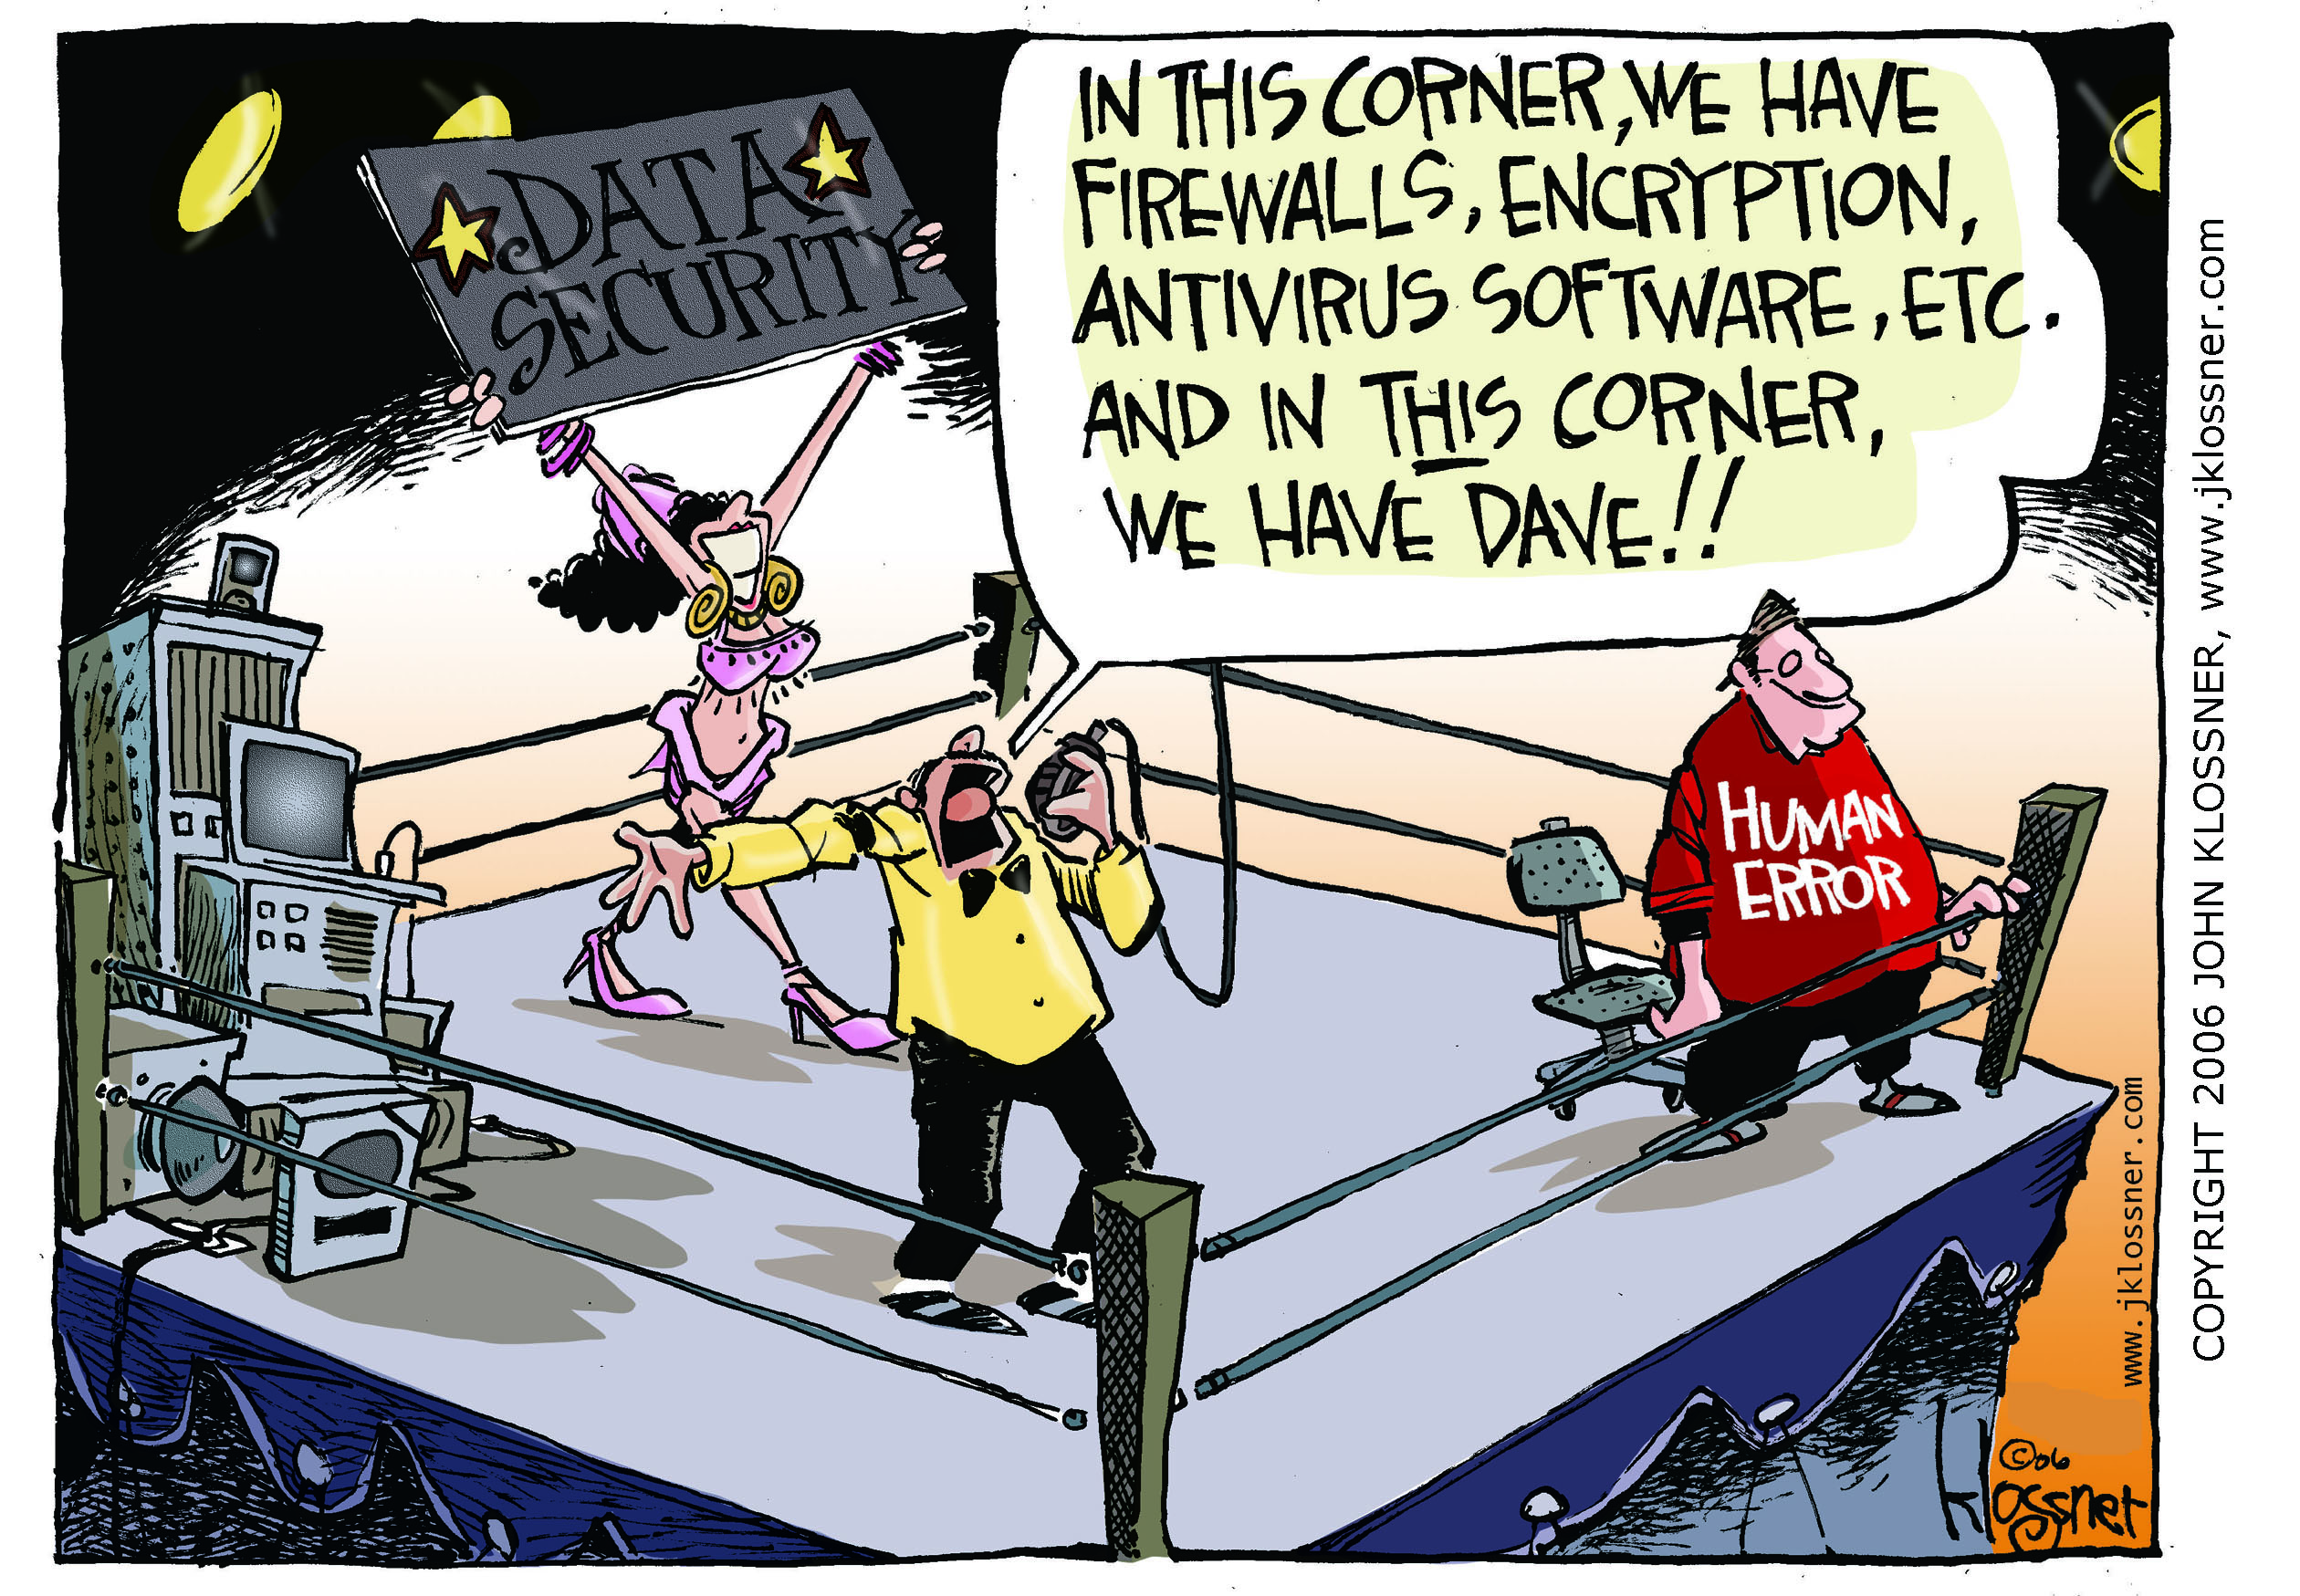
\includegraphics[width=\linewidth]{resources/cartoon_human_error.jpg}
  \caption[``Human Error'']{``Human Error'' - courtesy of John Klossner}
\end{figure}


% TODO:

% Het feit dat in essentie een nieuwe taal was, bracht ook een bijkomende
% leercurve met zich mee. Ook zorgde voortschrijdend inzicht voor stapsgewijze
% verbeteringen aan bepaalde constructies, die echter soms door tijdbeperkingen
% niet voor alle overige code konden bijgewerkt worden.

